\documentclass[11pt]{article}

\usepackage{fullpage}
\usepackage{graphicx}

\title{Heterogeneous Network Simulator Design Review}
\author{Matthew Leeds\\
	Tyler Allen\\}
\date{\today}

\begin{document}
\maketitle

\noindent \textbf{Abstract}

While the Internet was originally designed for computers with stable connections that rarely changed location, the number of mobile devices online has grown rapidly over the past few years. If access to the Internet were a single homogeneous network, this would not pose an issue, but the landscape of wireless access technologies has become more diverse, with WiFi, 3G/4G cellular networks, and WiMax often overlapping. Because of this environment, devices frequently have multiple options for how to connect to the Internet, but not enough information to know which connection would maximize throughput for them or for all devices competing for bandwidth. In theory, a Global Resource Controller (GRC) which has knowledge of all devices' bandwidth demands and connection options could allocate devices to networks in an optimal way. More specifically, the GRC could be configured to attempt to maximize the total throughput of all devices, to use a Max-Min Fair algorithm that prevents well-connected devices from hogging bandwidth, or some other configuration. We seek to create a simulation of just such an environment in order to further understanding of these systems, and potentially for use as an educational tool.

\section{Software Structure}

\begin{center}
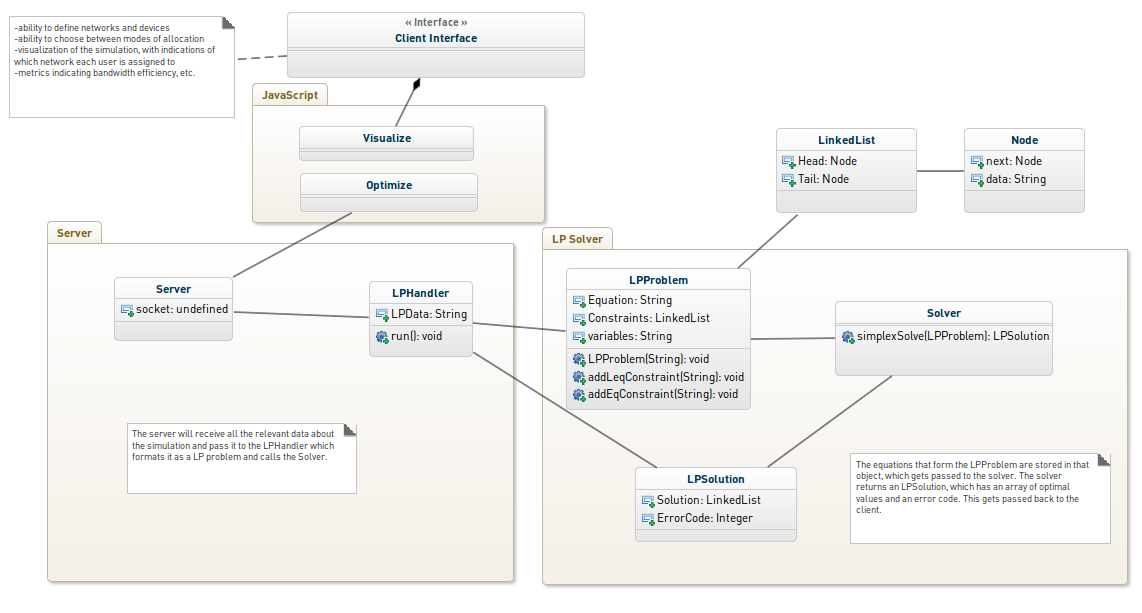
\includegraphics[width=600px, angle=270]{model.png}
\end{center}

\section{Implementation of the Linear Programming Solver}

details on the solver

\section{Questions}

questions

\section{Further Work}

more to be done

\end{document}
